% Command to problem header section
% Parameters {Problem Name}{Entrada estándar}{Salida estándar}{Time Limit}{Memory Limit (default 64 megabytes)}{Author}{Hedaxecimal Color (defaul white)}
\problemText{Mejor Trayecto}{Entrada estándar}{Salida estándar}{2 segundos}{}{Edu Sánchez}{FFFFFF}

Cusco es una ciudad turística llena de historia y belleza, con una gran cantidad de lugares para visitar. Para facilitar la planificación de los turistas, la ciudad dispone de un mapa detallado que muestra cómo recorrer la principales 4 atracciones.

% Includes the figures, with the necessary information about your problem
\begin{figure}[h]
    \centering
    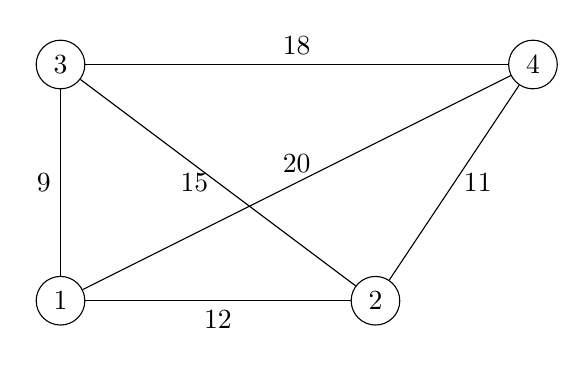
\begin{tikzpicture}
 \node[circle,draw] (A) at (0,0) {1};
 \node[circle,draw] (B) at (4,0) {2};
 \node[circle,draw] (C) at (0,3) {3};
 \node[circle,draw] (D) at (6,3) {4};

 \draw (A) -- node[midway, below] {12} (B); 
 \draw (A) -- node[midway, left] {9} (C);
 \draw (A) -- node[midway, above] {20} (D);
 \draw (B) -- node[midway, left] {15} (C);
 \draw (B) -- node[midway, right] {11} (D);
 \draw (C) -- node[midway, above] {18} (D); 
\end{tikzpicture}

    \captionsetup{labelformat=empty}
    \caption{Lugares turísticos y distancias.}
\end{figure}

Tus amigos extranjeros están visitando Cusco y quieren encontrar el trayecto más largo de la ciudad para visitar exactamente 4 lugares túristicos sin repetir ninguno, recorriendo exactamente tres caminos. ¿Puedes ayudarlos con esta tarea?

% Command to input text section
\inputText

La primera línea contiene un número entero $t (1 \leq t \leq 1000)$,  que indica el número de casos de prueba.

Cada caso de prueba incluye 6 líneas, las distancias entre cada par de lugares. Cada línea incluye tres números enteros $a, b$ y $d$, $(1 \leq a < b \leq 4, 1 \leq d \leq 1000)$, los dos primeros números identifican el número del lugar turístico y el tercer número la distancia entre los dos lugares.

% Command to output text section
\outputText

Imprime un único número entero, el trayecto más largo para visitar los 4 lugares turísticos.

% Command to examples section
\exampleCases

% Create a table with some examples of input and output cases
% Parameters {Example case filepath}
\begin{example}
    \exmp{%%INPUT
        \caseFile{template/MejorTrayectoEnCusco/in/1.in}
    }{%%OUTPUT
        \caseFile{template/MejorTrayectoEnCusco/out/1.out}
    }%%END-OUTPUT
\end{example}

% Command to explanation section, If you need to clarify anything from the example cases
\explanationText

En el primer ejemplo tus amigos tienen que visitar las ciudades en e orden $1, 4, 3$ y $2$ para tener la mayor distancia. Siendo el trayecto máximo de 53 unidades.
